\chapter{Machine Learning Model Review}
\label{ch2}

\section{Fundamentals of Training and Testing}
\begin{figure}[h!]
	\centering
		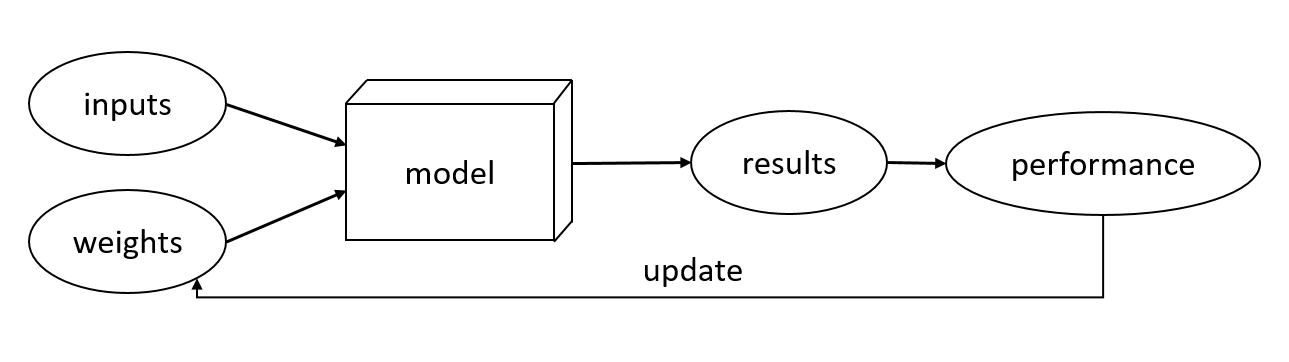
\includegraphics[width=0.99\textwidth]
		{training_process.png}
		\hfill
		\caption{Simple example of machine learning model training .}
		\label{fig:simple_model_training}
\end{figure}

\begin{figure}[h!]
	\centering
	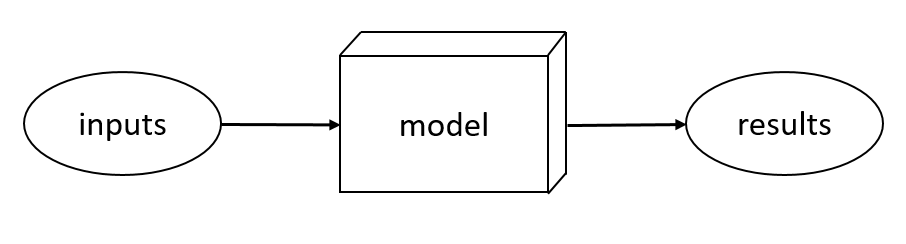
\includegraphics[width=0.99\textwidth]
	{testing_process.png}
	\hfill
	\caption{Simple example of machine learning model testing.}
	\label{fig:simple_model_testing}
\end{figure}

%\begin{figure}[h!]
%	\centering
%	\subfloat[Training\label{fig:simple_model_training_testing_a}]{
%		\includegraphics[width=0.99\textwidth]
%		{training_process.png}
%	}
%	\hfill
%	\subfloat[Testing\label{fig:simple_model_training_testing_b}]{
%		\includegraphics[width=0.99\textwidth]
%		{testing_process.png}
%	}
%	\hfill
%	\caption{Simple example of machine learning model training and testing.}
%	\label{fig:simple_model_training_testing}
%\end{figure}

\section{MLP and RNN Architectures}